%---------DO NOT EDIT THIS INDENTED SECTION
	% Preamble
	\documentclass[11pt,reqno,oneside,a4paper]{article}
	\usepackage[a4paper,includeheadfoot,left=35mm,right=35mm,top=00mm,bottom=30mm,headheight=40mm]{geometry} %sets up the margins
	\usepackage{graphicx}
	\usepackage{hyperref}
	\usepackage{booktabs}
	\graphicspath{{./images/}}
	\setlength{\parindent}{0pt}
	%%%%%%%%%%%%%%%%%%%%%%%%%%%%%%%%%%%%%%%%%%%%%%%%%%%%%%%%%%%%%%%%%%%%%%%%%%%%%%%%
%
% This file contains some standard modifications to basic LaTeX2e and
% the article documentclass. DO NOT EDIT THIS FILE, but do look through
% and make use of the shorthands defined herein.
%
%%%%%%%%%%%%%%%%%%%%%%%%%%%%%%%%%%%%%%%%%%%%%%%%%%%%%%%%%%%%%%%%%%%%%%%%%%%%%%%%

% Standard packages
\usepackage{amssymb,amsmath,amsthm}
\usepackage{xcolor,graphicx}
\usepackage{verbatim}
\usepackage{hyperref}
% Layout of headers & footers
\usepackage{titling}
\usepackage{fancyhdr}
\pagestyle{fancy} \lhead{{\theauthor}} \chead{} \rhead{} \lfoot{} \cfoot{\thepage} \rfoot{}

% Hyphenation
\hyphenation{non-zero}

% Instructor's email address
\newcommand{\InstEmail}{fspagnuolo@yale-nus.edu.sg}

%% Mathmode shortcuts
% Number sets
\newcommand{\NN}{\mathbb N}              % The set of naturals
\newcommand{\NNzero}{\NN^0}              % The set of naturals including zero
\newcommand{\NNone}{\NN}                 % The set of naturals excluding zero
\newcommand{\ZZ}{\mathbb Z}              % The set of integers
\newcommand{\QQ}{\mathbb Q}              % The set of rationals
\newcommand{\RR}{\mathbb R}              % The set of reals
\newcommand{\CC}{\mathbb C}              % The set of complex numbers
\newcommand{\KK}{\mathbb K}              % An arbitrary field
% Modern typesetting for the real and imaginary parts of a complex number
\renewcommand{\Re}{\operatorname*{Re}} \renewcommand{\Im}{\operatorname*{Im}}
% Upright d for derivatives
\newcommand{\D}{\ensuremath{\,\mathrm{d}}}
% Make epsilons look more different from the element symbol
\renewcommand{\epsilon}{\varepsilon}
% Always use slanted forms of \leq, \geq
\renewcommand{\geq}{\geqslant}
\renewcommand{\leq}{\leqslant}
% Shorthand for some relations
\newcommand{\po}{\preceq}
\newcommand{\rel}{{\mathcal R}} \newcommand{\rels}{\mathbin{\scriptstyle{\mathcal R}}}
% Shorthand for "if and only if" symbol
\newcommand{\Iff}{\ensuremath{\Leftrightarrow}}
% Make bold symbols for vectors
\providecommand{\BVec}[1]{\mathbf{#1}}
% Barred forms of \oplus and \otimes to represent the descents of these binary operators
\newcommand{\oplusbar}{\mathbin{\ooalign{$\hidewidth\overline{\oplus}\hidewidth$\cr$\phantom{\oplus}$}}} \newcommand{\otimesbar}{\mathbin{\ooalign{$\hidewidth\overline{\otimes}\hidewidth$\cr$\phantom{\otimes}$}}}
% Mathematical operators used in Proof
\DeclareMathOperator{\sgn}{sgn}          % The signum of a real number
\DeclareMathOperator{\power}{\mathcal{P}} % The power set of a set
\DeclareMathOperator{\Id}{Id}            % The identity function
\DeclareMathOperator{\Fun}{Fun}          % The set of functions from one set to another
\DeclareMathOperator{\Perm}{Perm}        % The set of permutations on a set
\DeclareMathOperator{\GCD}{GCD}          % The greatest common divisor of two integers
\newcommand{\abs}[1]{\left\lvert#1\right\rvert} % The absolute value of a real number or modulus of a complex number, with automatically scaling delimiters
 % Use the standard texHead for this module. You should not edit this file.
	%%%%%%%%%%%%%%%%%%%%%%%%%%%%%%%%%%%%%%%%%%%%%%%%%%%%%%%%%%%%%%%%%%%%%%%%%%%%%%%%
%
% This file contains some standard modifications to basic LaTeX2e and
% the article documentclass. DO NOT EDIT THIS FILE, but do look through
% and make use of the shorthands defined herein.
%
% This file should be input only after texHead-Proof-Standard.tex,
% specifically after the line
% \usepackage{amssymb,amsmath,amsthm}
% of that file.
%
%%%%%%%%%%%%%%%%%%%%%%%%%%%%%%%%%%%%%%%%%%%%%%%%%%%%%%%%%%%%%%%%%%%%%%%%%%%%%%%%

% Theorem definitions in the amsthm standard
\newtheorem{thm}{Theorem}
\newtheorem{lem}[thm]{Lemma}
\newtheorem{sublem}[thm]{Sublemma}
\newtheorem{prop}[thm]{Proposition}
\newtheorem{cor}[thm]{Corollary}
\newtheorem{conc}[thm]{Conclusion}
\newtheorem{conj}[thm]{Conjecture}
\theoremstyle{definition}
\newtheorem{defn}[thm]{Definition}
\newtheorem{cond}[thm]{Condition}
\newtheorem{asm}[thm]{Assumption}
\newtheorem{ntn}[thm]{Notation}
\newtheorem{prob}[thm]{Problem}
\theoremstyle{remark}
\newtheorem{rmk}[thm]{Remark}
\newtheorem{eg}[thm]{Example}
\newtheorem*{hint}{Hint}
 % Use the standard theorem definitions for this module. You should not edit this file.
	%---The following code defines the title, author, and date of the document.
	\title{Applying Explainable AI techniques to the APP-350 Corpus - MCS MidTerm Capstone Report}
	\date{\today}   % Using \today automatically updates to the document's build date
%----------------------------------
%---------IF YOU WANT TO DEFINE YOUR OWN MACROS, YOU CAN DO SO HERE ...

%---------... TO HERE

\author{Tristan Koh} 

\begin{document}
\maketitle
\thispagestyle{fancy}

%-----------EDIT FROM HERE

\begin{abstract}
	This is the for the capstone project YSS4107 under the double degree law and liberal arts program. It is also intended to fulfil the MCS major capstone requirements. The code can be found \href{https://github.com/TristanKoh/capstone-repo}{here}.
\end{abstract}

\section{Definitions}

\begin{itemize}
	\item Explainable AI is a branch of AI that seeks to explain the predictions of machine learning models through statistical explanations and visualisations.
	\item Natural Language Processing (NLP) is a subset of machine learning that aims to quantifiably analyse natural language. 
	\item APP-350 Corpus is a corpus of 350 Android app privacy policies annotated with privacy practices (i.e. behaviour that can have privacy implications). 
\end{itemize}

\section{Objective of capstone}
Using Interpret Text, I aim to train a machine learning model using the APP-350 corpus to predict the type of privacy practices within app privacy policies. I then use Interpret Text tools to visualise why the model made such predictions from a machine learning perspective. I then compare and contrast this with how a lawyer would reason about the privacy policy.

\section{Rationale of capstone}
Natural language forms the bread and butter of the legal industry, as expressed in contracts, judgements and legislation. There has been an increasing trend within the legal industry to adopt more machine learning techniques to automate and assist low level legal analysis. Within the specific context of data privacy, it would be useful to have a tool that assesses the possible data privacy risks of user policies. Such a tool would naturally use NLP techniques. Nevertheless, these tools should still be accessible to the layperson lawyer that might not be trained in data science.

\bigskip

While NLP techniques have substantially increased in performance in recent years, it has come at the cost of explainability of predictions because of the usage of neural networks which are architecturally more complex than traditional machine learning models. This lack of explainability of neural networks could potentially be a significant hindrance towards their adoption within the legal industry because the lawyer / law firm which uses these models still ultimately bear the responsibility of ensuring that the analysis is legally sound. 

\bigskip

However, the intersection in skillset between data science and legal analysis is still nascent and it is unrealistic to expect all legally trained personnel to be trained in data science to the extent required to interpret the predictions of machine learning models without aid.

\bigskip
Recent research within the legal NLP space have focused on building higher performing models and Text representation, but there have been comparatively few papers that assess the explainability of such models. Therefore, my capstone aims to bridge the gap between the lawyer and the data scientist by using Explainable AI techniques to explain the predictions of machine learning models in the context of predicting data privacy practices of app policies.

\section{Explanation of Dataset ("The APP-350 corpus")}

The APP-350 Corpus consists of 350 annotated Android app privacy policies. Each annotation consists of a practice and a modality.

\bigskip

A "privacy practice" (or "practice") describes a certain behaviour of an app that can have privacy implications (e.g., collection of a phone's device identifier or sharing of its location with ad networks). There are two modalities: PERFORMED (i.e. a practice is explicitly described as being performed) and NOT\_PERFORMED (i.e. a practice is explicitly described as not being performed).

\bigskip

As not all practices had modalities, altogether, 57 different categories were annotated. The following is a table of the practices and their descriptions.

\pagebreak

\begin{table}[]
	\resizebox{\textwidth}{!}{%
	\begin{tabular}{ll}
	\hline
	Data Type                 & Description                                                                                    \\ \hline
	Contact                   & The policy describes collection of unspecified contact data.                                   \\
	Contact\_Address\_Book    & The policy describes collection of contact data from a user's address book on the phone.       \\
	Contact\_City             & The policy describes collection of the user's city.                                            \\ 
	Contact\_E\_Mail\_Address & The policy describes collection of the user's e-mail.                                          \\
	Contact\_Password         & The policy describes collection of the user's password.                                        \\
	Contact\_Phone\_Number    & The policy describes collection of the user's phone number.                                    \\
	Contact\_Postal\_Address  & The policy describes collection of the user's postal address.                                  \\
	Contact\_ZIP              & The policy describes collection of the user's ZIP code.                                        \\
	Demographic               & The policy describes collection of the user's unspecified demographic data.                    \\
	Demographic\_Age          & The policy describes collection of the user's age (including birth date and age range).        \\
	Demographic\_Gender       & The policy describes collection of the user's gender.                                          \\
	Identifier                & The policy describes collection of the user's unspecified identifiers.                         \\
	Identifier\_Ad\_ID        & The policy describes collection of the user's ad ID (such as the Google Ad ID).                \\
	Identifier\_Cookie\_or\_similar\_Tech & The policy describes collection of the user's HTTP cookies, flash cookies, pixel tags, or similar identifiers. \\
	Identifier\_Device\_ID    & The policy describes collection of the user's device ID (such as the Android ID).              \\
	Identifier\_IMEI          & The policy describes collection of the user's IMEI (International Mobile Equipment Identity).  \\
	Identifier\_IMSI          & The policy describes collection of the user's IMSI (International Mobile Subscriber Identity). \\
	Identifier\_IP\_Address   & The policy describes collection of the user's IP address.                                      \\
	Identifier\_MAC           & The policy describes collection of the user's MAC address.                                     \\
	Identifier\_Mobile\_Carrier           & The policy describes collection of the user's mobile carrier name or other mobile carrier identifier.          \\
	Identifier\_SIM\_Serial   & The policy describes collection of the user's SIM serial number.                               \\
	Identifier\_SSID\_BSSID   & The policy describes collection of the user's SSID or BSSID.                                   \\
	Location                  & The policy describes collection of the user's unspecified location data.                       \\
	Location\_Bluetooth       & The policy describes collection of the user's Bluetooth location data.                         \\
	Location\_Cell\_Tower     & The policy describes collection of the user's cell tower location data.                        \\
	Location\_GPS             & The policy describes collection of the user's GPS location data.                               \\
	Location\_IP\_Address     & The policy describes collection of the user's IP location data.                                \\
	Location\_WiFi            & The policy describes collection of the user's WiFi location data.                              \\
	SSO                       & The policy describes receiving data from an unspecified single sign on service.                \\
	Facebook\_SSO             & The policy describes receiving data from the Facebook single sign on service.                 
	\end{tabular}%
	}
	\caption{List of annotated data privacy practices and their descriptions.}
	\end{table}


\bigskip

The APP-350 Corpus was used in a broader project to train machine learning models to conduct a privacy census of 1,035,853 Android apps. 
In that project, the researchers downloaded the data privacy practices of all apps from the Play Store with more than 350 million installs (which totalled 247 apps) and 103 randomly selected apps with 5 million installs. 
In total, the researchers collected the data privacy policies of 350 apps.

\bigskip

All 350 policies were annotated by one of the authors, a lawyer with experience in data privacy law. To ensure reliability of annotations, 2 other law students were hired to double annotate 10\% of the corpus. With a mean of Krippendorff's $\alpha = 0.78$\footnote{Krippendorff's $\alpha$ is a measure of agreement, with $\alpha > 0.8$ indicating good agreement, $0.67 <= \alpha <= 0.8$ indicating fair agreement, and $\alpha < 0.67$ indicating doubtful agreement.}, the agreement between the annotations exceeded previous similar research.

\bigskip

For more information about how the Corpus was annotated, see the paper “MAPS: Scaling Privacy Compliance Analysis to a Million Apps”, Section 3, Pg 69 to 70. 

\section{Rationale for utilising the APP-350 corpus} \label{sec:rationale-app350}

Since the focus of this capstone is to assess the interpretability of XAI models specifically within a legal context, this dataset was chosen for the following reasons:

\begin{enumerate}
	\item APP-350 contains real-world data privacy practices as they were scraped from Google PlayStore apps. Thus training XAI models on such a dataset would provide a realistic insight into the extent of which AI models are explainable in the legal context.
	\item Legal tech companies are also using such datasets to train models as part of their contract / document review products. By using APP-350 to train XAI models, the results can be used as a (simple)\footnote{The datasets used in industry are usually much larger and the models used are more complicated. However, APP-350 would be sufficiently complicated to serve as a toy example at an undergraduate level.} proxy for the explainability of models that are currently used in the industry.
	\item APP-350 is a labelled dataset, allowing easy validation of results. If an unlabelled dataset was used, unsupervised training would have to be conducted. The performance of the models would likely be much lower because NLP models for specific vocabulary like law are still not as sophisticated as models trained on general vocabulary. Further, there are few law specific labelled datasets to begin with. 
	\item APP-350 is labelled on both the sentence and segment (i.e. paragraph) level. This provides more granular data for training the AI models. 
\end{enumerate}

\section{Methodology}

There are three major steps to the capstone: First is data pre-processing, second is model training and applying XAI techniques to visualise their predictions ("Model Training and XAI visualisation"), and the last is to survey law and non-law students about whether they find these explanations interpretable ("Survey to assess interpretability"). I describe the specific methodology of these parts below.

\subsection{Data pre-processing}

The annotated privacy policies were originally in .yml format, with one .yml file containing one app data privacy policy. As explained above, each data privacy policy is labelled at both the sentence and segment level. The data was restructured from .yml to .csv, with one .csv file containing annotated sentences and the other containing annotated segments. By having two levels of text data for model training, this would provide another dimension to compare model performance on.

\subsection{Model training and XAI visualisation}

As the original researchers used the same dataset to train classifiers to predict on unseen data privacy policies, I adopt their training methodology and model choice as a guide for this capstone. 

\bigskip

The original researchers feature engineered the data as follows (Page 71 to 72): 

\begin{enumerate}
	\item Tokenisation: Lowercase all characters, remove non-ASCII characters, no stemming, normalisation of whitespace and punctuation, unigrams and bigrams.
	\item Word representation: Union of TF-IDF and manually crafted features. The manually crafted features consist of Boolean values indicating the presence or absence of indicative strings the researchers observed in the data.
\end{enumerate}

Individual classifiers were then trained for every policy classification. For all the classifications (except for four categories), they trained a model using the scikit-learn SVC implementation with a linear kernel, with five-fold cross validation. For the four policy classifications, word-based rule classifiers were used instead because of the limited number of training data.

(Add performance of researchers' models here.)

\subsubsection{Proposed model training methodology}

There are three main factors that I vary: Text representation, ML model, and XAI package used to explain the trained model.

\subsubsection{Text representation}

Computers cannot understand text directly and have to be converted into some kind of quantitative data. Therefore in NLP, text representations are methods to represent text as numeric or continuous vectors. This step is done before the model is trained. I use Tf-IDF (term frequency - inverse document frequency) and GloVe word embeddings as the text representations.

\bigskip

The Tf-IDF metric for a word in a document is calculated by multiplying two different metrics:

\begin{enumerate}
	\item Term frequency (TF) of a word in a document. This is the number of times the word appears in a document.
	\item Inverse document frequency (IDF) of the word across a set of documents. This is calculated by taking the total number of documents and dividing it by the number of documents that contain the specific word. This calculates the rarity of the term across all the documents. The closer the IDF of a word is to 0, the more common the word is.
\end{enumerate}

Mathematically, the Tf-IDF score for the word $t$ in the document $d$ from the document set $D$ can be stated as such:

\[tf-idf(t, d, D) = tf(t, d) \cdot idf(t, D)\]
where 
\begin{align*}
	tf(t, d) &= log(1 + freq(t, d )) \\
	idf(t, D) &= log\left(\frac{N}{count(d \in D : t \in d)}\right)
\end{align*}

\bigskip

While Tf-IDF is easy to calculate, one of its limitations is that it is a purely count-based metric. Tf-IDF does not take into account the context of the word. For example, Tf-IDF would not be able to capture the semantic relationship between words. Word embeddings try to overcome this issue with count-based metrics like Tf-IDF. Word embeddings are vector representation of words, such that the vectors closer to each other in a vector space are similar in their semantic meaning.\footnote{https://becominghuman.ai/mathematical-introduction-to-glove-word-embedding-60f24154e54c}

\bigskip

GloVe is one type of word embeddings (more information to be added)

\subsubsection{Model choice}
As the researchers found that the SVC classifier produces the best performance, I use SVC as well. In all, I use the following models:
\begin{enumerate}
	\item Logistic regression
	\item SGDClassifier
	\item SVC
	\item Ensemble classifiers (AdaBoost, GradientBoost, Random Forest)
\end{enumerate}

Logistic regression functions as a baseline classifier for its simplicity. SGDClassifier functions a possible alternative to SVC since the SGDClassifier can use a linear SVM loss function. Ensemble classifiers are included to provide a wider range of models to compare performance.

\bigskip

The two broad types of AI models that are usually used are classical machine learning models (such as logistic regression and tree-based classifiers) and neural networks. Though recent advances in NLP are in the field of neural networks \footnote{State of the art NLP models include BERT and ELMo.}, I chose to focus only on classical ML models to reduce the possible complexity of the capstone, as the field of NLP by itself produces models that are usually more complex than models trained on quantitative variables. Explaining neural networks used for NLP would be a much more complex task compared to explaining classical ML models.

Further, as the APP-350 corpus only contains (insert number here) datapoints, there is insufficient data to train neural networks. Generally, neural networks require (add number here) datapoints to perform well.

\subsubsection{XAI packages}
\begin{enumerate}
	\item LIME
	\item SHAP
	\item OmniXAI
	\item Interpret Text

	Interpret Text allows visualisation of the predictions of NLP models across a range of complexities. 

	\bigskip

	For linear and tree-based models, Interpret Text uses a Classical Text Explainer. The Explainer leverages this inherent explainability by exposing weights and importances over encoded tokens as explanations over each word in a document. In practice, these can be accessed through the visualization dashboard or the explanation object.

	\bigskip
	The explanations provided by the aforementioned glass-box methods serve as direct proxies for weights and parameters in the model, which make the final prediction.

\end{enumerate}

\subsection{Survey to assess interpretability}

To be added.

\section{Findings so far}

\subsection{Exploratory Data Analysis (EDA)}
As mentioned above, there are two levels of text data: Sentence level and segment level. As I train and compare the performance of models on both levels of data, I also conducted the EDA on both levels.

\subsubsection{Sentence level}
There are a total of 18829 annotated sentences. The table below shows some summary statistics of the top 10 and bottom 10 frequently occurring practices at the sentence level. 

\pagebreak

\begin{table}[]
	\resizebox{\textwidth}{!}{
	\begin{tabular}{lrrrr}
	\toprule
									  practice &  counts &  sentence\_length\_mean &  sentence\_length\_median &  counts\_percentage \\
	\midrule
	Identifier\_Cookie\_or\_similar\_Tech\_1stParty &    2107 &             25.389654 &                    22.0 &           11.2\% \\
			   Contact\_E\_Mail\_Address\_1stParty &    2106 &             28.651472 &                    25.0 &           11.2\% \\
							 Location\_1stParty &    1514 &             29.159181 &                    24.0 &           8.1\% \\
	Identifier\_Cookie\_or\_similar\_Tech\_3rdParty &    1250 &             27.318400 &                    24.0 &           6.6\% \\
				Identifier\_IP\_Address\_1stParty &    1005 &             30.913433 &                    27.0 &           5.3\% \\
				 Contact\_Phone\_Number\_1stParty &     970 &             29.117526 &                    25.0 &           5.2\% \\
				 Identifier\_Device\_ID\_1stParty &     697 &             32.377331 &                    28.0 &           3.7\% \\
			   Contact\_Postal\_Address\_1stParty &     597 &             28.907873 &                    26.0 &           3.2\% \\
										   SSO &     504 &             32.565476 &                    28.0 &           2.7\% \\
					  Demographic\_Age\_1stParty &     428 &             33.074766 &                    26.0 &           2.3\% \\
	\bottomrule
	\end{tabular}
	}
	\caption{Summary statistics for top 10 occurring practices at sentence level.}
	\end{table}

	\bigskip

	\begin{table}[]
		\resizebox{\textwidth}{!}{
		\begin{tabular}{lrrrr}
		\toprule
								practice &  counts &  sentence\_length\_mean &  sentence\_length\_median &  counts\_percentage \\
		\midrule
		Identifier\_Mobile\_Carrier\_3rdParty &      35 &             47.057143 &                    30.0 &           0.19\% \\
					Contact\_ZIP\_3rdParty &      34 &             40.176471 &                    41.0 &           0.18\% \\
		Identifier\_SSID\_BSSID\_1stParty &      33 &             28.060606 &                    24.0 &           0.18\% \\
			  Contact\_Password\_3rdParty &      33 &             24.181818 &                    20.0 &           0.18\% \\
					Contact\_City\_3rdParty &      24 &             18.000000 &                    14.0 &           0.13\% \\
		Contact\_Address\_Book\_3rdParty &      17 &             39.647059 &                    34.0 &           0.1\% \\
			  Identifier\_IMSI\_1stParty &      13 &             48.153846 &                    44.0 &           0.07\% \\
		Identifier\_SIM\_Serial\_3rdParty &       5 &             41.200000 &                    54.0 &           0.03\% \\
			  Identifier\_IMSI\_3rdParty &       4 &             54.250000 &                    47.5 &           0.02\% \\
		Identifier\_SSID\_BSSID\_3rdParty &       2 &             65.500000 &                    65.5 &           0.01\% \\
		\bottomrule
		\end{tabular}
		}
		\caption{Summary statistics for bottom 10 frequently occurring practices.}
		\end{table}

\bigskip

In total, the top 10 frequently occurring practices make up approximately 60\% of the dataset. The bottom 10 frequently occurring practices make up approximately 1\% of the dataset.

\bigskip

According to Table 4 below, there does not seem to be much variation in sentence length for the top 10 frequently occurring practices, since the standard deviation for the mean is approximately 2.5 words and the median 1.9 words. This could indicate similar sentence complexity across the practices.

\begin{table}
	\centering
	\begin{tabular}{lrr}
		\toprule
		{} &  sentence\_length\_mean &  sentence\_length\_median \\
		\midrule
		count &             10.000000 &               10.000000 \\
		mean  &             29.747511 &               25.500000 \\
		std   &              2.468191 &                1.900292 \\
		min   &             25.389654 &               22.000000 \\
		25\%   &             28.715572 &               24.250000 \\
		50\%   &             29.138353 &               25.500000 \\
		75\%   &             32.011357 &               26.750000 \\
		max   &             33.074766 &               28.000000 \\
		\bottomrule
		\end{tabular}
		\caption{Summary sentence statistics for top 10 frequently occurring practices.}
	\end{table}
	
\pagebreak

\subsubsection{Segment level}
There are in total 21623 segments. However, there are 11422 segments without any annotated practice. Hence there are 10201 annotated segments. The table below shows some summary statistics of the top 10 and bottom 10 frequently occurring practices at the segment level.

\begin{table}[htb]
	\resizebox{\textwidth}{!}{
	\begin{tabular}{lrrrr}
	\toprule
									  practice &  counts &  segment\_length\_mean &  segment\_length\_median &  counts\_percentage \\
	\midrule
			  Contact\_E\_Mail\_Address\_1stParty &    1105 &            84.118552 &                   72.0 &              10.83 \\
	Identifier\_Cookie\_or\_similar\_Tech\_1stParty &     858 &            81.913753 &                   68.5 &               8.41 \\
							Location\_1stParty &     821 &            89.794153 &                   70.0 &               8.05 \\
				Identifier\_IP\_Address\_1stParty &     590 &            96.984746 &                   73.0 &               5.78 \\
				Contact\_Phone\_Number\_1stParty &     565 &            90.371681 &                   67.0 &               5.54 \\
	Identifier\_Cookie\_or\_similar\_Tech\_3rdParty &     524 &           100.339695 &                   86.5 &               5.14 \\
				Identifier\_Device\_ID\_1stParty &     446 &            96.704036 &                   72.0 &               4.37 \\
			  Contact\_Postal\_Address\_1stParty &     364 &            85.598901 &                   69.5 &               3.57 \\
										  SSO &     274 &            99.463504 &                   86.5 &               2.69 \\
					  Demographic\_Age\_1stParty &     259 &            96.200772 &                   80.0 &               2.54 \\
	\bottomrule
	\end{tabular}
	}
	\caption{Summary statistics of top 10 frequently occurring practices by segment.}
  \end{table}

  \begin{table}[htb]
	\resizebox{\textwidth}{!}{
	\begin{tabular}{lrrrr}
	\toprule
							  practice &  counts &  segment\_length\_mean &  segment\_length\_median &  counts\_percentage \\
	\midrule
			  Identifier\_IMEI\_3rdParty &      23 &           115.347826 &                   93.0 &               0.23 \\
	Identifier\_Mobile\_Carrier\_3rdParty &      21 &           142.000000 &                  130.0 &               0.21 \\
			Contact\_Password\_3rdParty &      18 &            70.555556 &                   65.0 &               0.18 \\
		Identifier\_SSID\_BSSID\_1stParty &      16 &            86.062500 &                   71.0 &               0.16 \\
		Contact\_Address\_Book\_3rdParty &      14 &           296.928571 &                   78.5 &               0.14 \\
			  Identifier\_IMSI\_1stParty &      11 &            92.363636 &                   78.0 &               0.11 \\
				Contact\_City\_3rdParty &       8 &           100.500000 &                  104.0 &               0.08 \\
		Identifier\_SIM\_Serial\_3rdParty &       3 &            85.333333 &                   65.0 &               0.03 \\
			  Identifier\_IMSI\_3rdParty &       3 &            62.333333 &                   65.0 &               0.03 \\
		Identifier\_SSID\_BSSID\_3rdParty &       2 &           105.500000 &                  105.5 &               0.02 \\
	\bottomrule
	\end{tabular}
	}
	\caption{Summary statistics for bottom 10 frequently occurring practices.}
  \end{table}

The top 10 practices make up approximately 57\% of the dataset. The bottom 10 practices make up approximately 1.2\% of the dataset.

\bigskip

According to Table 7 below, there does not seem to be much variation in sentence length for the top 10 frequently occurring practices, since the standard deviation for the mean is approximately 6.7 words and the median 7.2 words. This could indicate similar segment complexity across the practices.

\pagebreak

\begin{table}[htb]
	\centering
	\begin{tabular}{lrr}
	\toprule
	{} &  segment\_length\_mean &  segment\_length\_median \\
	\midrule
	count &            10.000000 &              10.000000 \\
	mean  &            92.148979 &              74.500000 \\
	std   &             6.683275 &               7.230337 \\
	min   &            81.913753 &              67.000000 \\
	25\%   &            86.647714 &              69.625000 \\
	50\%   &            93.286227 &              72.000000 \\
	75\%   &            96.914568 &              78.250000 \\
	max   &           100.339695 &              86.500000 \\
	\bottomrule
	\end{tabular}
	\caption{Summary segment statistics for top 10 frequently occurring practices.}
  \end{table}

\subsection{Performance of classifiers for top N practices}
As seen in Table 2 and Table 5 above, there is an uneven distribution of records across the practices. Further, the bottom 10 frequently occurring practices for both sentence and segment level only contains about 2 to 35 records for each practice. Given that there are in total 57 practices for the entire dataset, and there is not a uniform distribution of occurrences. Training models on all 57 practices would likely lead to low performance since there are not enough records for all 57 practices. Thus, to find an optimal balance between model performance and still maintain a realistic sample of practices that could appear in a real world dataset, I chose to assess model performance by first assessing the performance of the models for the top N (where $3<= N <= 10$) frequently occurring practices at both the sentence and segment level.

\bigskip
I use Logistic Regression, SGDClassifier and SVC classifiers and compare the weighted precision, recall and F1 scores. Precision, Recall and F1 scores different metrics are used to assess the performance of classifiers. They are stated mathematically below.

\begin{align*}
	\text{Precision} &= \frac{\text{True Positive}}{\text{True Positive + False Positive}} \\
	\text{Recall} &= \frac{\text{True Positive}}{\text{True Positive + False Negative}} \\
	\text{F1} &= 2 \cdot \frac{\text{Precision} \cdot \text{Recall}}{\text{Precision + Recall}}
\end{align*}

Generally, precision is the preferred metric when the cost of false positives are high, such as detecting spam. If a classifier classifies a non-spam email as spam, the user would lose important information. Whereas recall is preferred when the costs of false negatives are high. For example, if a classifier classifies someone as not having cancer when they actually have cancer, the patient would lose the opportunity for early intervention. F1 is a harmonic mean of precision and recall, and is usually used to find a balance between precision and recall. Since there is neither a high cost for false positives or false negatives, F1 score is primarily used to assess the performance across the top N practices. As the distributions of records across the practices are uneven, I focus on the weighted average of F1 scores.

I also assess the top N performance for both the Tf-IDF and GLoVe word embeddings.

\subsubsection{Sentence level performance - Tf-IDF}

Generally we see that the SVC classifier performance the best across the metrics and across the top N frequently occurring practices. This corresponds with the findings by the researchers as they also found that the SVC classifier produced the best performance.

\begin{figure}[htb]
	\centering
	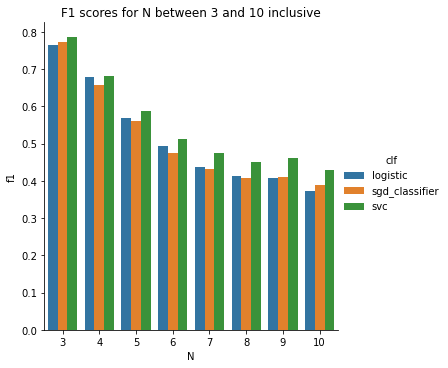
\includegraphics[width = 10cm]{sentence_f1.png}
	\caption{F1 scores for classifiers for top N occurring practices at sentence level}
\end{figure}

\begin{figure}[htb]
	\centering
	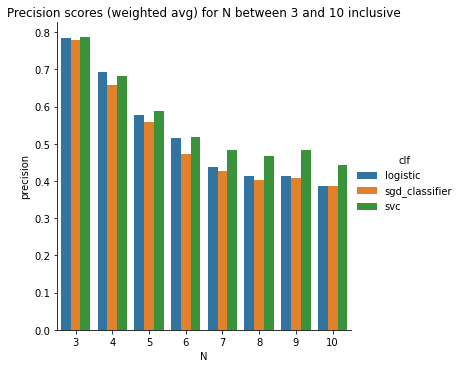
\includegraphics[width = 10cm]{sentence_precision.png}
	\caption{Precision scores for classifiers for top N occurring practices at sentence level}
\end{figure}

\begin{figure}[htb]
	\centering
	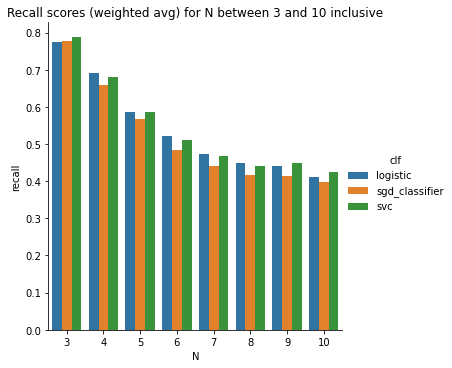
\includegraphics[width = 10cm]{sentence_recall.png}
	\caption{Recall scores for classifiers for top N occurring practices at sentence level}
\end{figure}

\subsubsection{Sentence level performance - Word embeddings}

\subsubsection{Segment level performance - Tf-IDF}

\subsubsection{Segment level performance - Word embeddings}



\subsection{Performance of individual classifiers for top 5 practices}

\subsection{XAI visualisation of models}

\section{Further steps to take in Semester 2}

\end{document}
